


In \cref{fig:evolution}, we generated similarity plots for the various sites over five eras in order to see how well our groupings based on chemical composition map on to connections posited by historians and archeologists based on a much larger set of data. Because our data comes from a fairly long historical period, we needed to break it up into eras in order to have a well-defined set of historical theories and connections with which to compare it. That is, historians are not generally in the business of theorizing about the connection between Mycenae and Palaiokastro over the entire bronze age, but over much smaller periods. 



\begin{figure}
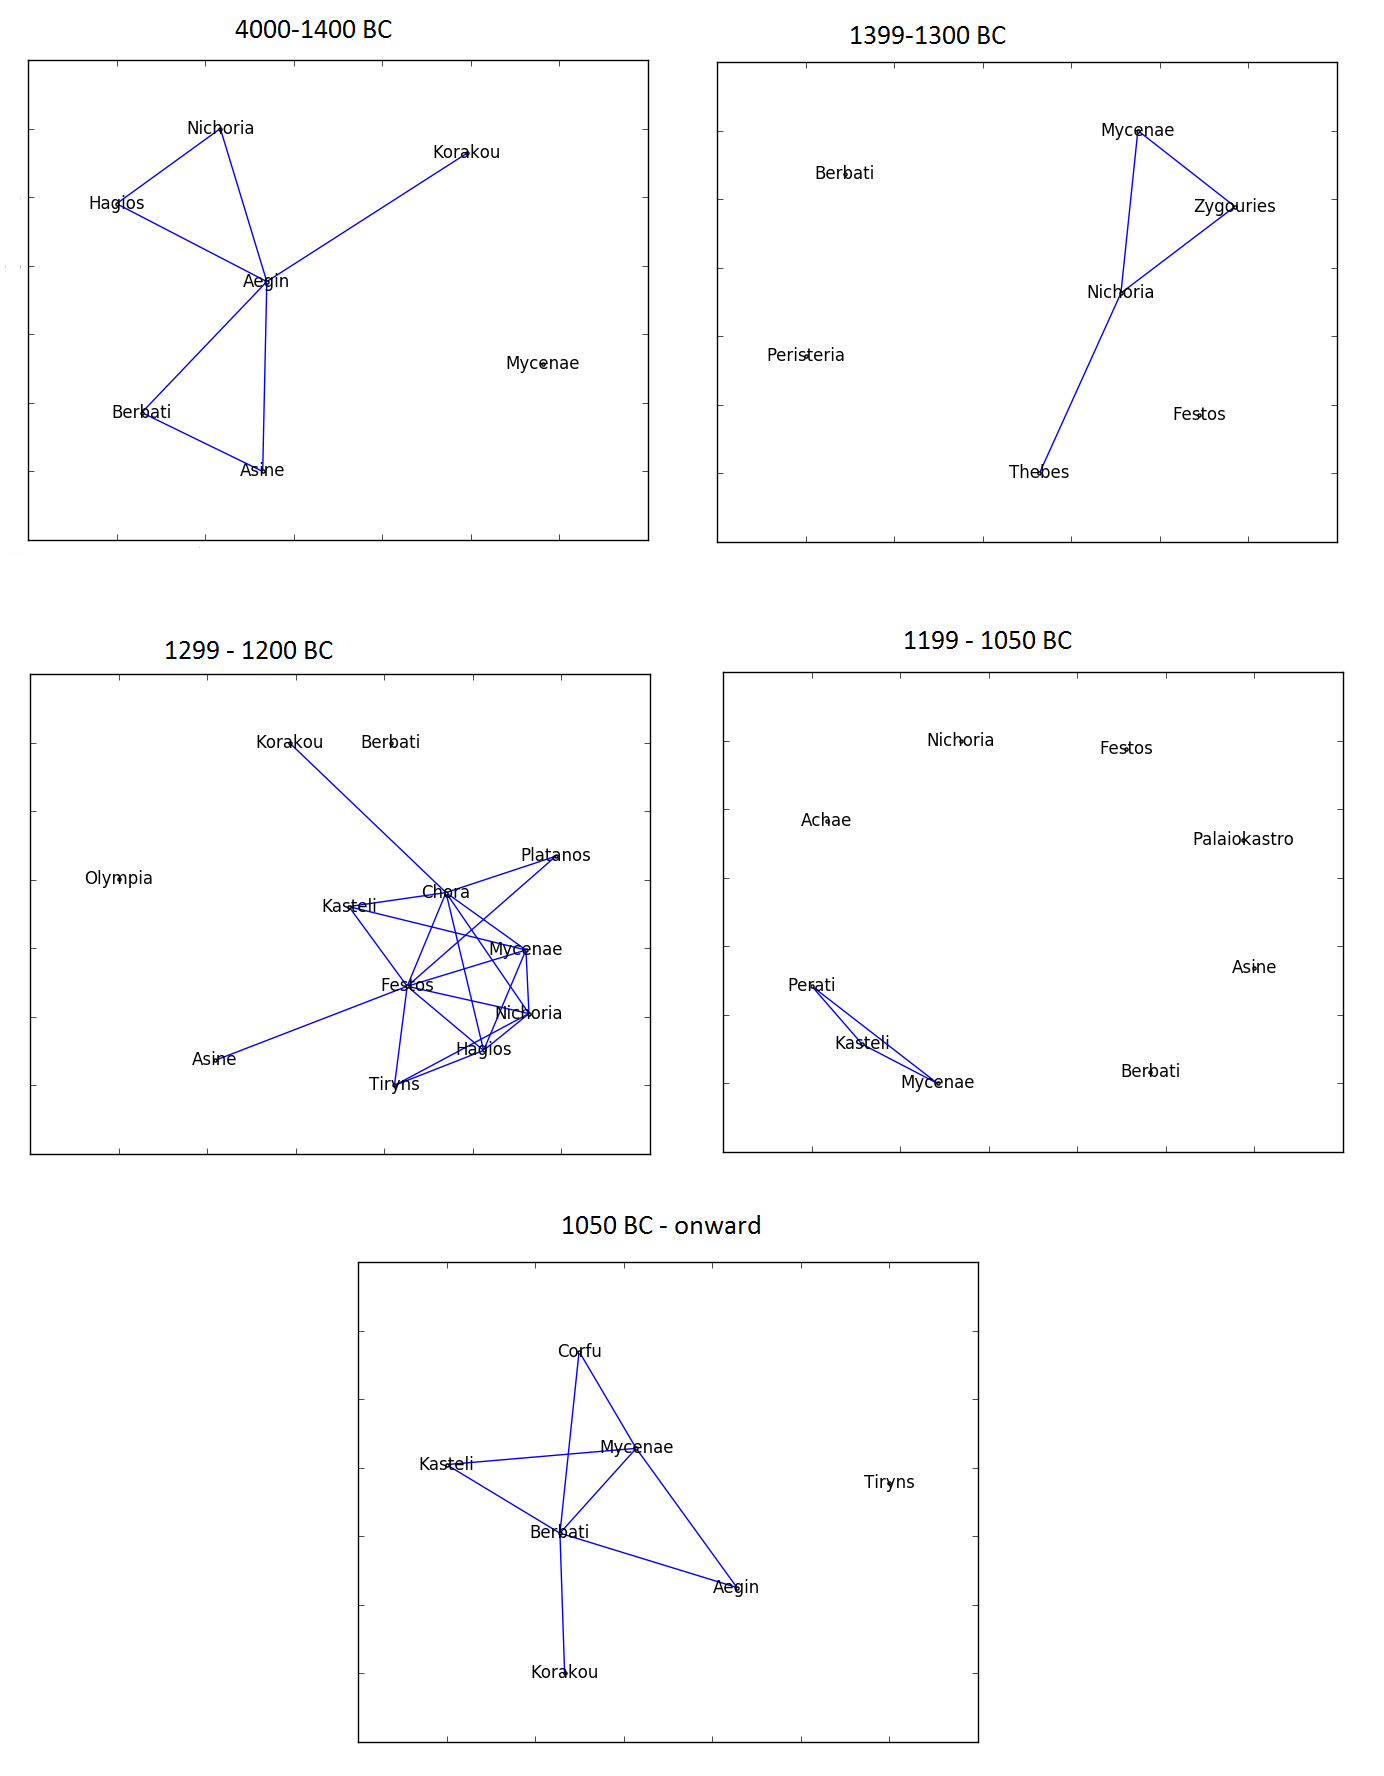
\includegraphics[width=\textwidth]{Network_evolution.png}
\caption{Evolution of networks of the Archaeological sites}
\label{fig:evolution}
\end{figure}


We chose periods 2-4 based on the standard chronology for bronze age Greece displaying in \cref{fig:timeline}: period 2 (1399-1300) is the Late Helladic III-A, period 3 (1299-1200) is the Late Helladic III-C, and period 4 (1199-1050) is the Late Helladic III-C. The first period includes the earliest artifacts in the dataset; we allowed a much larger period because there were fewer sites and artifacts from this era, and likewise with the final period, which includes artifacts up to Roman times. 
  
  How many sites in each period?
  
In \cref{fig:evolution}, every site with artifacts dating from that period was included in the graph for that period. The blue links show a kernel-based similarity in the sites based on those artifacts, as described in SECTION. Every similarity measure over a threshold is represented. We chose this threshold based on the histogram of the sum number of connections according to each possible threshold: $10^{5}$ was selected since it was near the median across all eras.

One way of analyzing these plots is to look at the most connected site in each era, that is, the site with the most number of links. A link between sites could represent either geographic factors or cultural-historical ones. Geographic factors include similarity in raw materials available at those sites, either due to proximity or similarity in geographic features such as altitude or distance from bodies of water. Cultural-historical factors include trade, influence and other forms of resettling, conflict and movement of people. For instance, artifacts could reflect trade relations in their chemical composition by actually sharing an origin if they were produced in one site and traded to another, or more indirectly by reflecting similar styles in material, such as a trend in red ware that spread via cultural influence rather than the literal trade in red ware pots.  Note that many stylistic features would not be represented in chemical composition, such as drawings and figures which are often used to track influence \cite{hruby2010mycenaean}.Thus, the most connected site is an indication of some kind of centrality or similarity, but a priori it is hard to predict what kind of similarity would show up in chemical composition.

The first thing to notice about \cref{fig:evolution} is that the connection between sites change significantly throughout the eras. In fact no two recurring sites retain a link in all graphs where they both appear. Of course, geographical proximity between sites does not change over time, nor does altitude, or proximity to water and natural resources (for the most part). This alone indicates that our similarity measure is not determined by these geographic factors. 

Starting in era 1, we see that Aegine is the most connected site, linked to 5 others whereas the next most connected sites are only linked to 2 others. Aegine was a powerful city in the middle Bronze age, so this is not surprising - though there are relatively few artifacts and a long period here so not much can be safely inferred. 

In era 2, the Late Helladic III-A, Nichoria is the most connected, with 3 links, followed by Zygouries and Mycenae with 2.  Nichoria is already theorized to have been paticularly prominent in III-A and III-B\cite{shelmerdine1981nichoria}, and even though it has artifacts represented in era 4, it does not have any links. The entire late Helladic-III is thought to be characterized by Mycenean dominance\cite{demand2011mediterranean}, and it is in this period that Mycenae starts to be among the most connected nodes in our graph. 

Era 3 encompasses the Late Helladic III-B period, the high period of the Mycenaen trade network \cite{demand2011mediterranean}. 

Era 4 has less connectivity, even relative to the number of sites represented, with only a triad of Perati-Mycenae-Kasteli Chania. This could be indirectly due to the fact that this marks the beginning of the dark age. A reduction in economic power and trade could lead to fewer relations between cities and thereby more local cohesion. Alternately, the 

Era 5 again shows a cluster containing Mycenae towards the center, along with Berbati. 

Overall, 

 
  




\begin{figure}
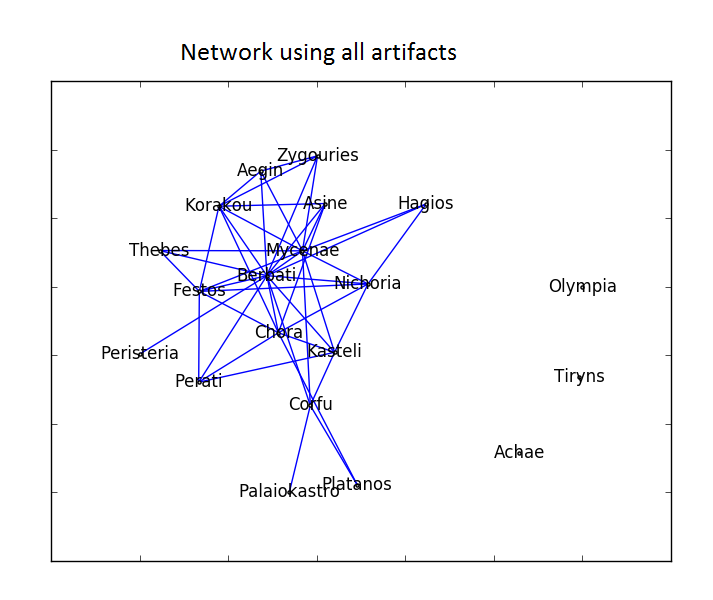
\includegraphics[width=\textwidth]{Overall_Network.png}
\caption{Overall network of the Archaeological sites}
\label{fig:overall}
\end{figure}


\begin{figure}
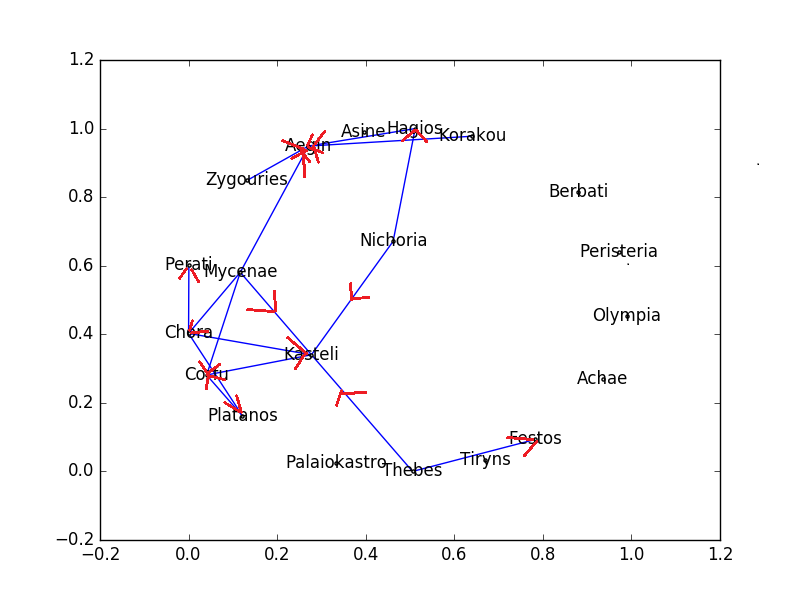
\includegraphics[width=\textwidth]{Overall_network_direct.png}
\caption{Directed network of the Archaeological sites}
\label{fig:overall}
\end{figure}
